\documentclass[10pt,a4paper]{article}
\usepackage[utf8]{inputenc}
\usepackage[russian]{babel}
\usepackage[OT1]{fontenc}
\usepackage{amsmath}
\usepackage{amsfonts}
\usepackage{amssymb}
\usepackage{graphicx}
\author{Никитина А.В, Замотаева Ю.И.}
\title{Отчет\\ по лабораторным работам по дисциплине " Телекоммуникационные системы и сети"}
\begin{document}
\maketitle
\pagebreak
\tableofcontents
\pagebreak

\section{Линейная фильтрация}
\subsection{Цель работы}
Изучить воздействия ФНЧ на тестовый сигнал с шумом. Сгенерировать гармонический сигнал с шумом и синтезировать ФНЧ. Получить сигнал во временной и частотной областях до и после фильтрации.
\subsection{Ход работы}
Линейный фильтр — динамическая система, применяющая некий линейный оператор ко входному сигналу для выделения или подавления определённых частот сигнала и других функций по обработке входного сигнала. 
Фильтр Баттерворта — один из типов электронных фильтров. Фильтры этого класса отличаются от других методом проектирования. Фильтр Баттерворта проектируется так, чтобы его амплитудно-частотная характеристика была максимально гладкой на частотах полосы пропускания. 

 В командном окне Matlab сгенерируем гармонический сигнал без шума и с шумом, а также спектры сигнала с шумом и без шума. В результате код Matlabа будет выглядеть так:
\begin{verbatim}
x = 0:0.01:4*pi;
f=100*(0:255)/512;
figure
noise=rand(size(x));
y = sin(2*pi*x);
y_noisy = y+0.3*noise;

%Построение сигнала без шума:
plot(x(1:200),y(1:200))
grid

%Построение сигнала с шумом:
plot(x(1:200),y_noisy(1:200))
grid

%синтез ФНЧ Баттерворта
[B,A] = butter(16,0.99);
B=B./sum(B);
A=A./sum(A);
%обработка сигнала ФНЧ
figure
y_filtered = conv(y_noisy,[B,A]);

%Построение сигнала после прохождения через фильтр:
plot(x(1:200),y_filtered(1:200))
grid
figure
%Построение спектра сигнала с шумом
noisy_spectrum = fft(y_noisy,512);
norm_noisy_spectrum = noisy_spectrum.*conj(noisy_spectrum)/512;

%Построение нормирова спектра сигнала с шумом:
plot(f,norm_noisy_spectrum(1:256))
axis([0 max(f) 0 2])
grid
figure

%Спектр отфильтрованного сигнала
spectrum = fft(y_filtered,512);
norm_filtered_spectrum=spectrum.*conj(spectrum)/512;
%Построение нормированого отфильтрованного спектра:
plot(f,norm_filtered_spectrum(1:256))
axis([0 max(f) 0 2])
grid
\end{verbatim}
Результаты работы программы на рис.13.
\begin{figure}[H]
\begin{minipage}[h]{0.6\linewidth}
\center{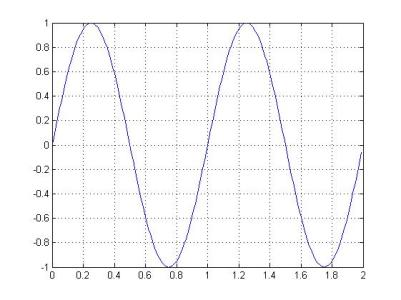
\includegraphics[width=1\linewidth]{im1}} a) \\
\end{minipage}
\vfill
\begin{minipage}[h]{0.6\linewidth}
\center{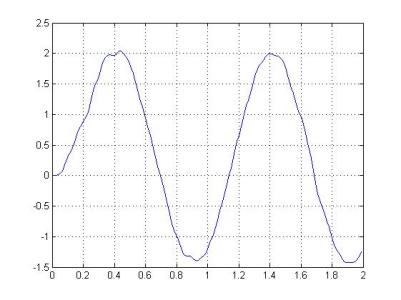
\includegraphics[width=1\linewidth]{im2}} \\б)
\end{minipage}
\hfill
\begin{minipage}[h]{0.6\linewidth}
\center{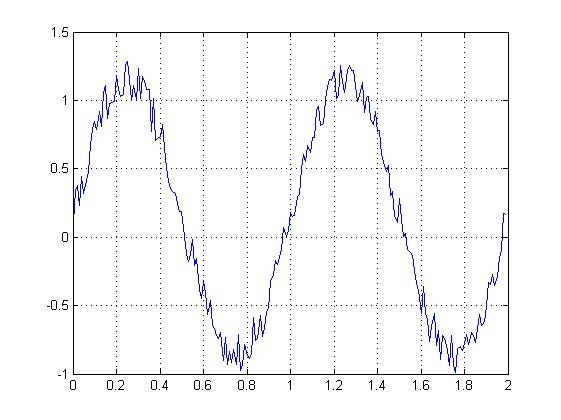
\includegraphics[width=1\linewidth]{im56}} в) \\
\end{minipage}

\vfill
\begin{minipage}[h]{0.6\linewidth}
\center{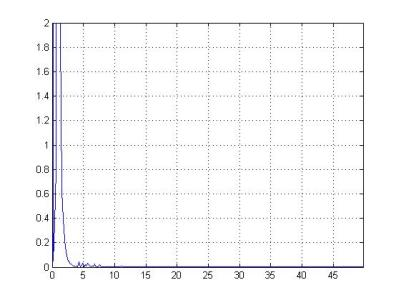
\includegraphics[width=1\linewidth]{im4}} г) \\
\end{minipage}
\hfill
\begin{minipage}[h]{0.6\linewidth}
\center{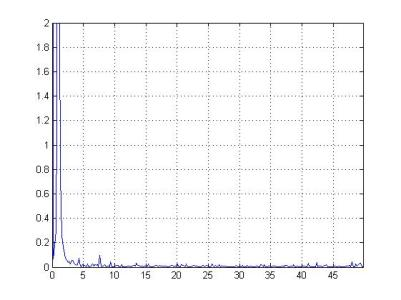
\includegraphics[width=1\linewidth]{im3}} д) \\
\end{minipage}
\caption{Линейная фильтрация в Matlab: a) Сигнал без шума, б)
Сигнал после фильтрации, в)Сигнал с шумом, г)Спектр сигнала после фильтрации, д)Спектр сигнала с шумом.}
\label{ris:experimentalcorrelationsignals}
\end{figure}
Для создания модели в Simulink используем блок Discrete FIR Filter раздела Discrete главной библиотеки и блок Digital Filter design из Signal Processing Blockset/Filtering/Filter Designs. Результаты моделирование в Simulink на рис.14.
\begin{figure}[H]
\begin{minipage}[h]{0.6\linewidth}
\center{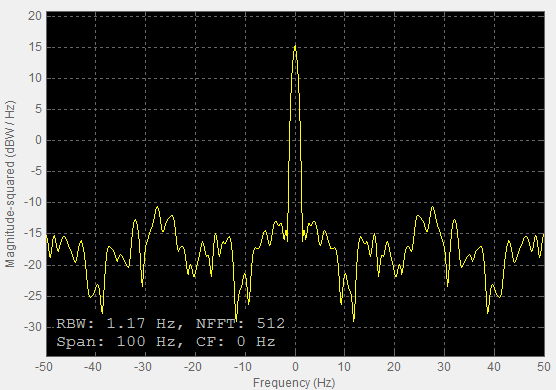
\includegraphics[width=1\linewidth]{im7}} a) \\
\end{minipage}
\hfill
\begin{minipage}[h]{0.6\linewidth}
\center{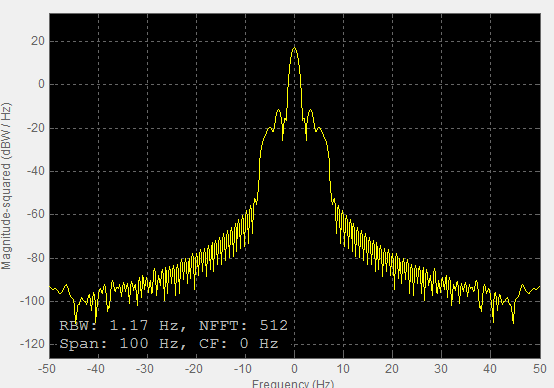
\includegraphics[width=1\linewidth]{im6}} \\б)
\end{minipage}
\vfill
\begin{minipage}[h]{0.6\linewidth}
\center{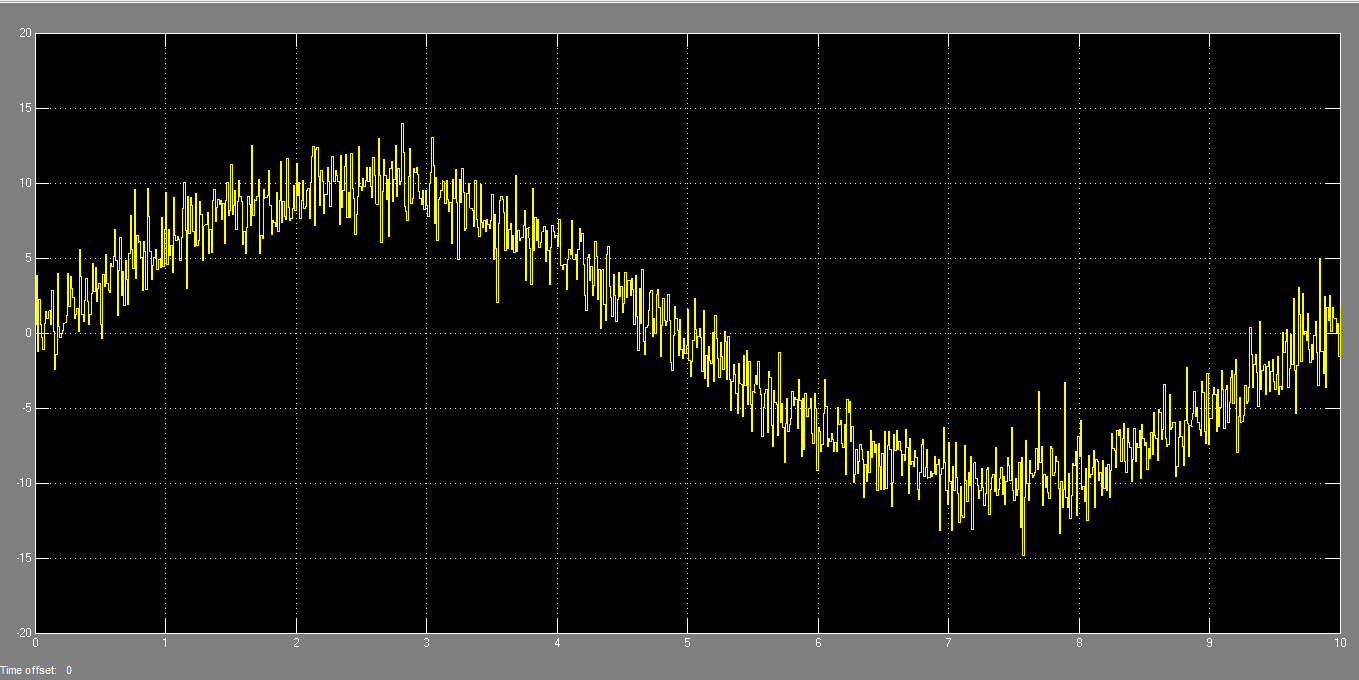
\includegraphics[width=1\linewidth]{im8}} в) \\
\end{minipage}
\hfill
\begin{minipage}[h]{0.6\linewidth}
\center{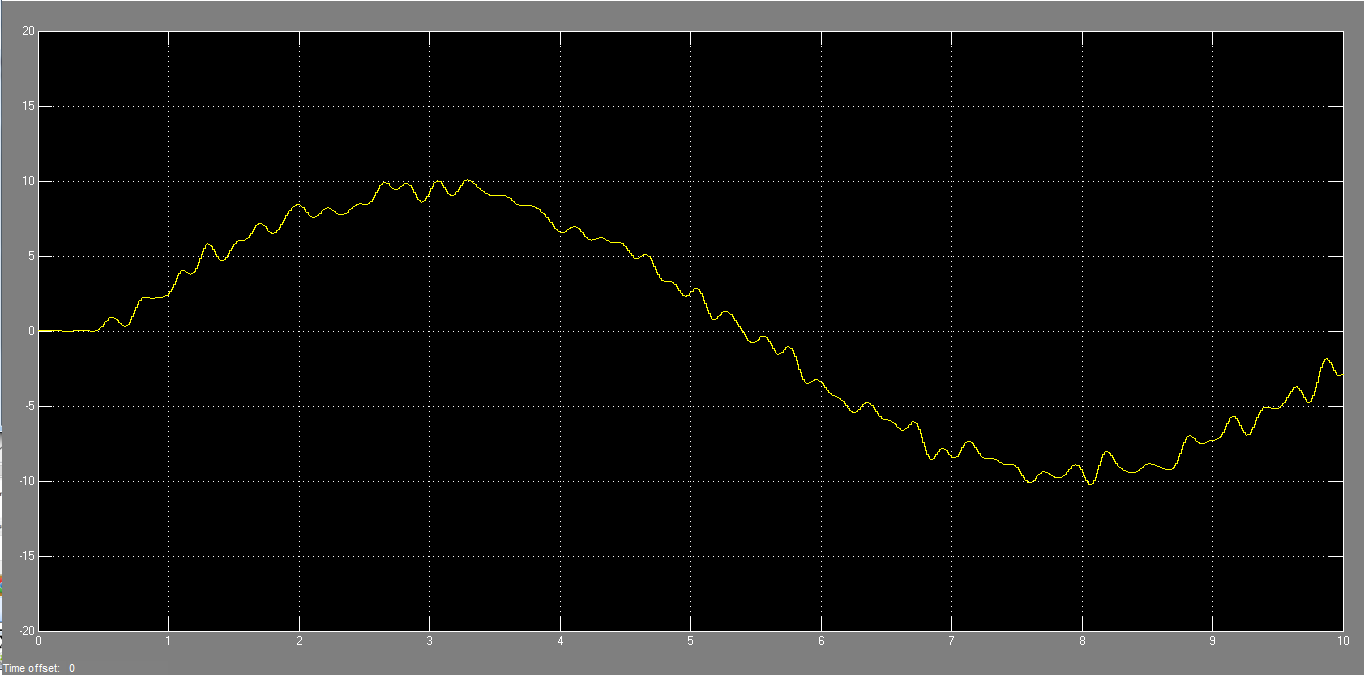
\includegraphics[width=1\linewidth]{im9}} г) \\
\end{minipage}
\hfill
\begin{minipage}[h]{0.6\linewidth}
\center{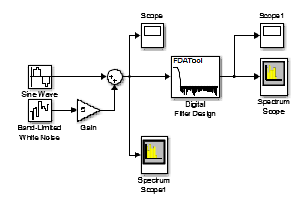
\includegraphics[width=1\linewidth]{im5}} д) \\
\end{minipage}
\caption{Линейная фильтрация в Simulink: a) Спектр до фильтрации, б)
Спектр после фильтрации, в)Сигнал до фильтрации, г)Сигнал после фильтрации, д) Схема модели.}
\label{ris:experimentalcorrelationsignals}
\end{figure}
\subsection{Вывод}
Фильтр нижних частот — один из видов аналоговых или электронных фильтров, эффективно пропускающий частотный спектр сигнала ниже некоторой частоты (частоты среза), и уменьшающий (подавляющий) частоты сигнала выше этой частоты. Степень подавления каждой частоты зависит от вида фильтра. В лабораторной работе мы произвели неполное удаление шума линейным фильтром. Для его полного удаления нам необходим идеальный фильтр (с прямоугольным окном). Линейная фильтрация не устраняет полностью шум, т.к. для полного удаления необходим идеальный фильтр с прямоугольным окном, которого на практике не существует. Так же, т. к. линейный фильтр подавляет все сигналы, находящиеся в его полосе задержания и не изменяет сигналы из полосы пропускания, то он не может удалить шум, который попал в его полосу 
пропускания. Соответственно удалить весь шум он не в силах. 

\end{document}